\documentclass[varwidth]{standalone}

\usepackage{amsmath}
\usepackage[dvipsnames]{xcolor}
\usepackage{tikz}
\usetikzlibrary{arrows.meta}
\usetikzlibrary{backgrounds}
\usetikzlibrary{calc}
\usetikzlibrary{fit}
\usetikzlibrary{positioning}
\usetikzlibrary{patterns}
\usetikzlibrary{shapes}
\usetikzlibrary{shapes.misc}


\begin{document}

\resizebox{\textwidth}{!}{%
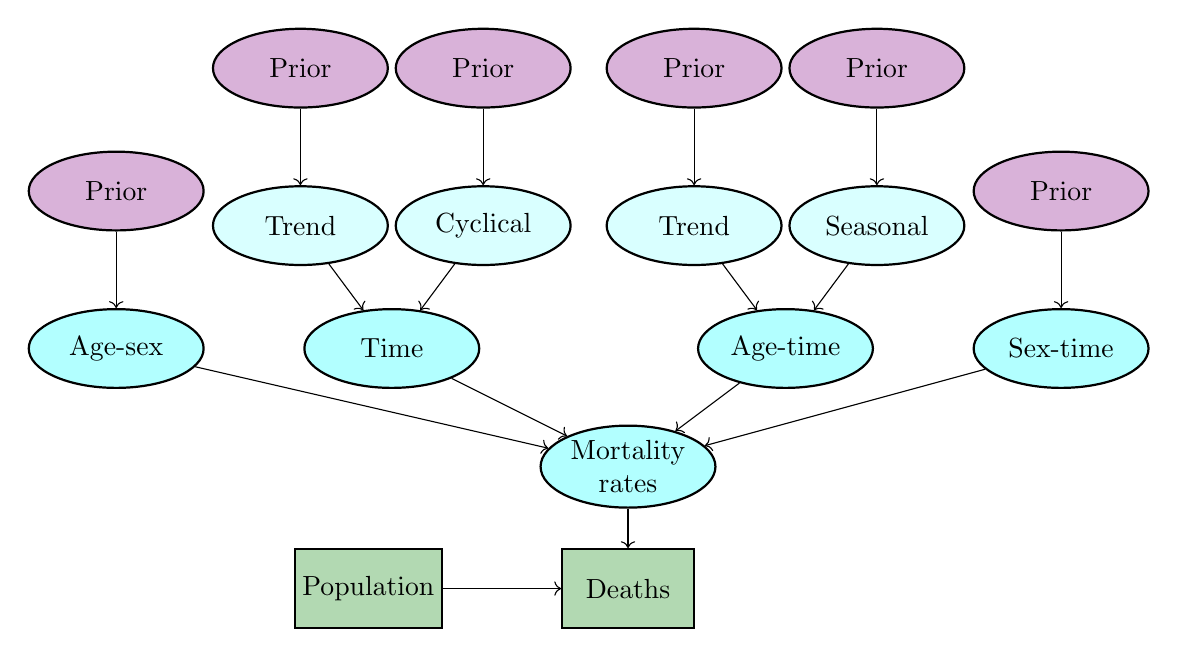
\begin{tikzpicture}
  [
    node distance = 1.5cm and 1.5cm,
    node/.style = {thick, draw, text width = 1.5cm,
                  minimum height = 1cm, align = center, inner sep = 1pt},
    obs/.style = {node, rectangle, text width = 1.6cm, fill=Green!30},
    unobs/.style = {node, ellipse, fill=Cyan!30},
    prior/.style = {unobs, fill=Purple!30},
    arrow/.style  = {> = stealth, thick, length=8pt},
  ]
    
  \node[obs] (y) {Deaths};
  \node[obs, text width = 1.8cm] [left = of y] (w) {Population}
  edge[->](y);

  \node[unobs][above = of y, yshift = -1cm] (mu) {Mortality rates}
    edge[->](y);

    \node[unobs] [above of = mu, xshift = -6.5cm, yshift = 0cm] (beta_agesex) {Age-sex}
      edge[->](mu);
    \node[unobs] [right of = beta_agesex, xshift = 2cm] (beta_time) {Time}
      edge[->](mu);
    \node[unobs] [right of = beta_time, xshift = 3.5cm] (beta_agetime) {Age-time}
      edge[->](mu);
    \node[unobs] [right of = beta_agetime, xshift = 2cm] (beta_sextime) {Sex-time}
      edge[->](mu);

    \node[prior] [above of = beta_agesex, yshift = 0.5cm] (pi_agesex) {Prior}
      edge[->](beta_agesex);
    \node[unobs,fill=Cyan!15] [above left of = beta_time, xshift = -0.1cm, yshift = 0.5cm] (trend_time) {Trend}
      edge[->](beta_time);
    \node[unobs,fill=Cyan!15] [above right of = beta_time, xshift = 0.1cm, yshift = 0.5cm] (cyclical_time) {Cyclical}
      edge[->](beta_time);
    \node[unobs,fill=Cyan!15] [above left of = beta_agetime, xshift = -0.1cm, yshift = 0.5cm] (trend_agetime) {Trend}
      edge[->](beta_agetime);
    \node[unobs,fill=Cyan!15] [above right of = beta_agetime, xshift = 0.1cm, yshift = 0.5cm] (season_agetime) {Seasonal}
    edge[->](beta_agetime);

    \node[prior] [above of = trend_time, yshift = 0.5cm] (pi_trend_time) {Prior}
      edge[->](trend_time);
    \node[prior] [above of = cyclical_time, yshift = 0.5cm] (pi_cyclical_time) {Prior}
      edge[->](cyclical_time);
    \node[prior] [above of = trend_agetime, yshift = 0.5cm] (pi_trend_agetime) {Prior}
      edge[->](trend_agetime);
    \node[prior] [above of = season_agetime, yshift = 0.5cm] (pi_season_agetime) {Prior}
      edge[->](season_agetime);

    \node[prior] [above of = beta_sextime, yshift = 0.5cm] (pi_sextime) {Prior}
      edge[->](beta_sextime);
      
  \end{tikzpicture}
  }
  \end{document}